\documentclass[12pt, a4paper]{article}
\usepackage[francais]{babel}
\usepackage{caption}
\usepackage{graphicx}
\usepackage[T1]{fontenc}
\usepackage{listings}
\usepackage{geometry}
\usepackage{minted}
\usepackage{array,multirow,makecell}
\usepackage[colorlinks=true,linkcolor=black,anchorcolor=black,citecolor=black,filecolor=black,menucolor=black,runcolor=black,urlcolor=black]{hyperref}
\setcellgapes{1pt}
\makegapedcells
\renewcommand{\listingscaption}{Code}

\begin{document}
\begin{titlepage}
    \begin{center}
        \vspace*{1cm}
 
        \textbf{\Large SAE 23 - Mettre en place une solution informatique pour l'entreprise}
 
      
             
        \vspace{6.5cm}
 
        \textbf{Fiche de procédure du déploiement\\
        de l'application sur serveur Apache}
 
        \vfill
             
       
             
        \vspace{3cm}
        Martin Baumgaertner\\
        IUT de Colmar\\
        17 juin 2022
    \end{center}
 \end{titlepage}
 \newpage
 \tableofcontents
 \newpage
 \section{Introduction}
    \subsection{Configuration de la machine}
    Pour commencer, j'ai choisi déployer mon application sur
    une machine sous Ubuntu Server. En effet, cette version est optimisée
    pour le type de déploiement que je vais effectuer. 
    J'ai donc installé les paquets suivants (nécessaires pour le déploiement) :
    \begin{listing}[H]
        \caption{Installation des paquets}
        \label{lst:paquets}
        \begin{minted}{bash}
        apt install python3-pip apache2 libapache2-mod-wsgi-py3
        \end{minted}
    \end{listing}
    Puis, j'ai configuré un environnement virtuel, dans lequel j'ai installé 
    tous les prérequis de mon projet (Django, Pillow, Django-crispy-forms, etc.):
    \begin{listing}[H]
        \caption{Configuration de l'environnement virtuel}
        \label{lst:environnement}
        \begin{minted}{bash}
        sudo apt install python3-venv
        python3 -m venv venv
        source venv/bin/activate
        pip3 install -r requirements.txt
        \end{minted}
    \end{listing}
    \subsection{Configuration des paramètres du projet}
    J'ai dû ajuster le fichier "settings.py" pour qu'il puisse être reconnu
    par Apache. 
    Premièrement, j'ai rajouté ces lignes de code :
    \begin{listing}[H]
        \caption{Rajout de l'adresse et du fichier de destination static}
        \label{lst:settings}
        \begin{minted}{bash}
        ALLOWED_HOSTS = ['webgrade.localhost']
        STATIC_ROOT = os.path.join(BASE_DIR, "static/")
        \end{minted}
    \end{listing}
    \newpage
\section{Serveur Apache}
    \subsection{Fichier de configuration du serveur Apache}
    Je suis aller créer un fichier du nom de mon projet donc "webgrade.conf" 
    Puis, je l'ai configuré en y insérant les lignes suivantes :
    \begin{listing}[H]
        \caption{Configuration du fichier webgrade.conf }
        \label{lst:conf}
        \begin{minted}{bash}
        sudo nano /etc/apache2/sites-available/webgrade.conf

        <VirtualHost *:80>
            ServerAdmin admin@webgrade.localhost
            ServerName webgrade.localhost
            ServerAlias www.webgrade.localhost
            DocumentRoot /home/martin/SAE-23
            ErrorLog ${APACHE_LOG_DIR}/error.log
            CustomLog ${APACHE_LOG_DIR}/access.log combined

            Alias /static /home/martin/SAE-23/static
            <Directory /home/martin/SAE-23/static>
                Require all granted
            </Directory>

            Alias /static /home/martin/SAE-23/media
            <Directory /home/martin/SAE-23/media>
                Require all granted
            </Directory>

            <Directory /home/martin/SAE-23/webgrade>
                <Files wsgi.py>
                    Require all granted
                </Files>
            </Directory>

            WSGIDaemonProcess SAE-23 python-path=/home/martin/SAE-23 
            python-home=/home/martin/SAE-23/env
            WSGIProcessGroup SAE-23
            WSGIScriptAlias / /home/martin/SAE-23/webgrade/wsgi.py
        </VirtualHost>
        \end{minted}
    \end{listing}
    \newpage
    Après la configuration du fichier, nous devons l'activer à l'aide
    de la 1ère commande puis, un message nous indique que nous devons 
    redémarrer les services Apache pour que la configuration prenne effet. 
    Ce que j'ai donc fait à l'aide de la deuxième commande : 
    \begin{listing}[H]
        \caption{Activation du fichier webgrade.conf }
        \label{lst:activer}
        \begin{minted}{bash}
        sudo a2ensite webgrade.conf

        service apache2 reload
        \end{minted}
    \end{listing}
    \subsection{Test de configuration}
    Pour vérifier que nous ne nous sommes pas trompés dans la configuration,
    nous pouvons taper cette commande à laquelle nous sera répondu comme message :
    "syntax OK" ce qui signifie donc qu'il n'y a pas d'erreur dans le fichier.
    \begin{listing}[H]
        \caption{Vérification de la configuration}
        \label{lst:verif}
        \begin{minted}{bash}
        sudo apache2ctl configtest 
        \end{minted}
    \end{listing}
\newpage
\section{Configuration de la base de données}
    \subsection{Création de la base de données}
    Pour mettre en place la base de données j’ai installé MariaDB-server 
    et client ainsi que MySQL. J’ai exporté la base de données que j’avais 
    créé sur ma machine hôte et je l’ai transféré sur ma machine Ubuntu.
    Ensuite, j’ai donc ouvert MariaDB et créé une base de données que j’ai 
    nommé « grade » à l’aide de la commande suivante : 
    \begin{listing}[H]
        \caption{Création de la base de données}
        \label{lst:db}
        \begin{minted}{sql}
        mysql -u root -p
        CREATE DATABASE grade;
        \end{minted}
    \end{listing}
    Puis, j’ai importé ma base de données déjà existante dans la
    nouvelle base de données que je viens de créer dans MariaDB avec
    cette commande, depuis le terminal linux : 
    \begin{listing}[H]
        \caption{Import de la base de données}
        \label{lst:import}
        \begin{minted}{sql}
        mysql -u root -p grade < grade.sql
        \end{minted}
    \end{listing}
    Pour pouvoir mettre en place la base de données avec le projet
    j’ai dû me connecter à la base de données que j’ai créée avec MariaDB,
    pour ce faire j’ai créé un utilisateur depuis MariaDB, et je lui ai
    donné tous les droits, à l’aide des commandes suivantes :
    \begin{listing}[H]
        \caption{Création de l'utilisateur avec tous les droits}
        \label{lst:user}
        \begin{minted}{sql}
        CREATE USER 'webgrade'@'localhost' IDENTIFIED BY 'webgrade';
        GRANT ALL PRIVILEGES ON *.* TO  'webgrade'@'localhost';
        \end{minted}
    \end{listing}
    \newpage
    Pour finir, j'ai renseigné les bons paramètres dans "database" dans le
    fichier settings.py de mon projet :
    \begin{listing}[H]
        \caption{Configuration de la base de données}
        \label{lst:database}
        \begin{minted}{python}
        DATABASES = {
            'default': {
                'ENGINE': 'django.db.backends.mysql',
                'NAME': 'grade',
                'USER': 'webgrade',
                'PASSWORD': 'webgrade',
                'HOST': 'localhost',
                'PORT': '3306',
            }
        }
        \end{minted}
    \end{listing}
\newpage
\section{Déployement de mon application}
Après avoir redémarré Apache, j’ai pu déployer mon application.
En me connectant depuis un navigateur et en saisissant l'adresse 
"webgrade.localhost" j'ai pu me connecter à mon application !
\begin{figure}[h]
    \centering
    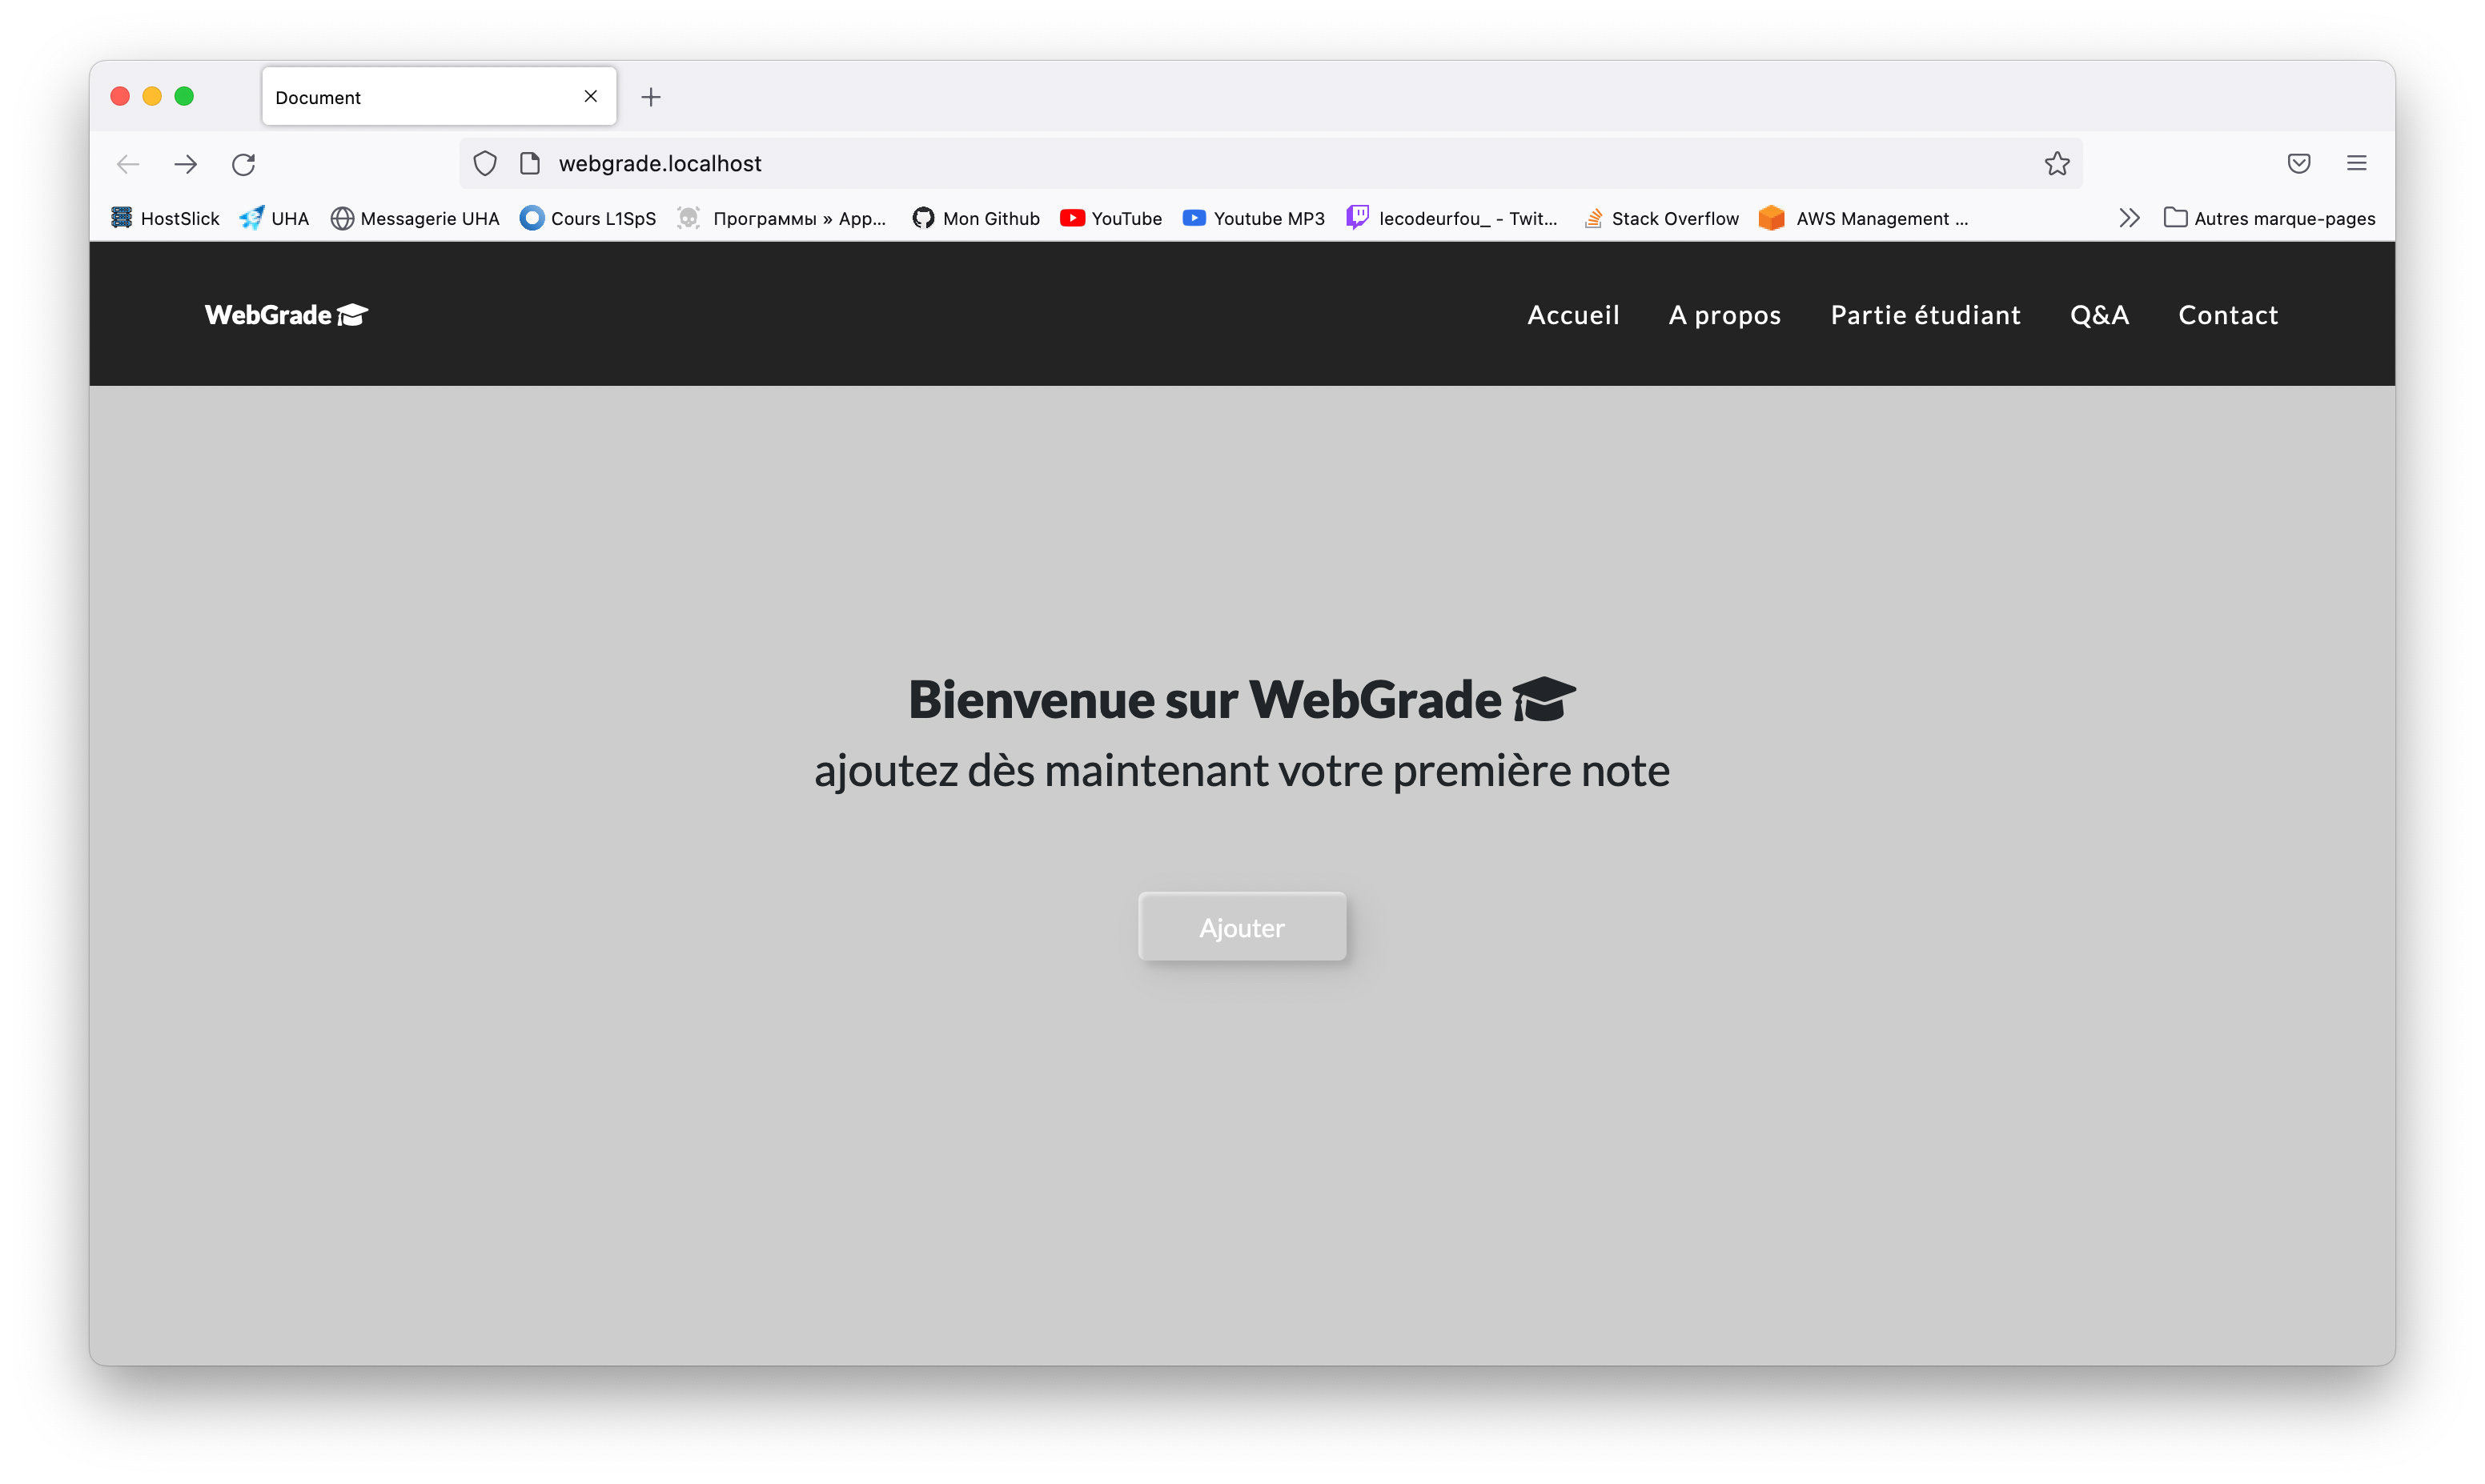
\includegraphics[width=1\textwidth]{webgrade.png}
    \caption{Notre application deployée sur le serveur !}
    \label{fig:dep}
\end{figure}
\end{document}